\clearpage
\section*{Raising the TS/tracker/LYSO assembly by 0.20 m}
All three trigger-scintillator (TS) stations, all four tracker sensors and both
LYSO layers move together by $+200$ mm in CAD $Z$. Their transverse positions,
rotations, internal spacings and segmentation stay the same. ECal and all three
HCal groups remain fixed. A muon must still cross every one of the 26 active layers.

\textbf{Raising this assembly alone reduces the estimated rate by 10.2\%.}
The top-TS to lower-LYSO separation stays at $383.4$ mm, preserving the internal
collimation, but the distance to the fixed, offset ECal grows by 200 mm. Fewer
accepted directions also cross every ECal layer. The geometric
$p>1\ \mathrm{GeV}/c$ reference changes from 1.0085 to
$0.9059\pm0.0003$ muons/hour; the error is numerical only.

\begin{center}
\begin{tabular}{lrrr}
\toprule
Overhead shielding & Original/hour & Raised/hour & Change\\
\midrule
None & 1.407 & 1.264 & $-10.2\%$\\
3 ft concrete & 1.199 & 1.077 & $-10.2\%$\\
\bottomrule
\end{tabular}
\end{center}

\subsection*{Centering the ECal as well}
Keep the TS/tracker/LYSO assembly raised and translate the entire ECal in $X,Y$
so that the centre of its combined active-silicon envelope lies on the LYSO/TS
axis. This means $\Delta X=+46.56$ mm and $\Delta Y=-46.08$ mm; ECal height,
rotations and internal layer offsets stay unchanged. All HCal positions stay fixed.
\textbf{Centering increases the rate by 54.2\% relative to raising alone},
and by 38.5\% relative to the original layout.

\begin{center}
\begin{tabular}{lrrr}
\toprule
Overhead shielding & Raised + centred/hour & Per day & Gain over raised\\
\midrule
None & 1.949 & 46.8 & $+54.2\%$\\
3 ft concrete & 1.660 & 39.8 & $+54.2\%$\\
\bottomrule
\end{tabular}
\end{center}

\begin{center}
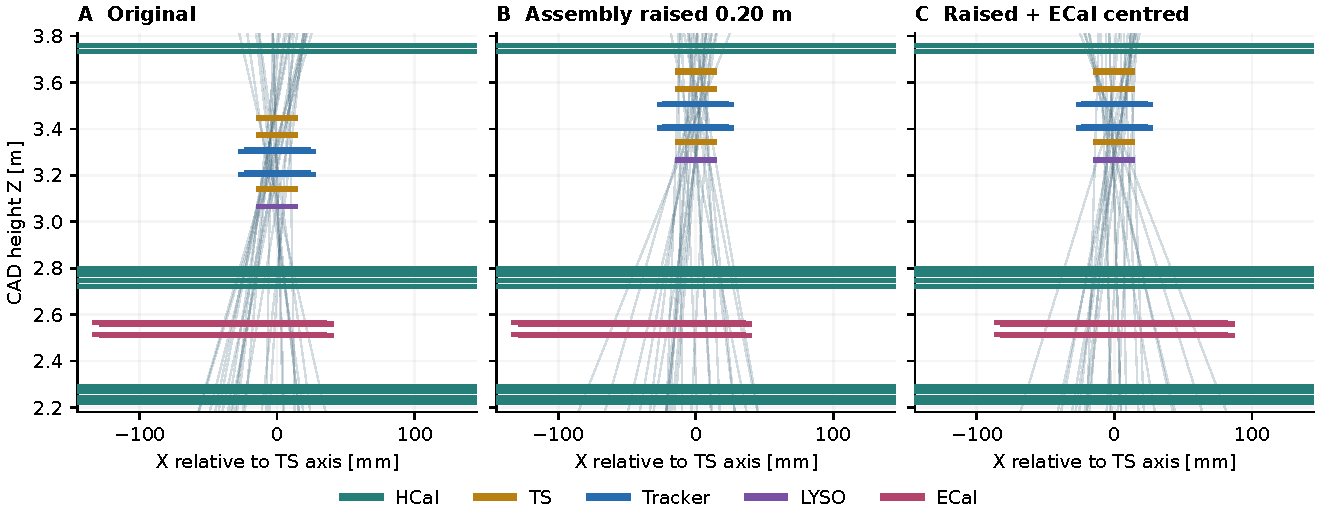
\includegraphics[width=\linewidth]{shift_up_200mm/geometry_shift_comparison.pdf}
\end{center}
\textbf{Figure 3.} The three layouts with 24 accepted straight rays each, in
$X$--$Z$. TS, tracker and LYSO move upward together in B and C; ECal is also
centred in C. Its $Y$ shift is not visible in this projection. Line thicknesses
are enlarged, and HCal extends outside the transverse window.

\textbf{Checks and limits.} Each variation uses eight Sobol scrambles of $2^{18}$
trials. ROOT agrees with all 4,992 layer decisions in each 192-ray test, including
109 translated active solids for B and 113 for C. Both independent pseudorandom
checks agree within 0.16 numerical standard errors. The spectrum and roof
model are unchanged. To isolate placement effects, the detector stopping proxy
stays at the original $32.70\ \mathrm{g\,cm^{-2}}$ vertical column; it is not
remeasured. Scattering, detector inefficiency and mechanical clearances remain
unmodelled. These are rate studies, not validated mechanical or transport geometries.

